\chapter{Preliminaries}

\section{Vector spaces, norms, and scalar products}
\begin{defn}[Vector space]\label{preliminaries:defn:vectorspace}
    A vector space over a field $\mathbb{F}$ is a set $V$ with two operations $+:\mathbb{F}\times V\rightarrow V$, $(u,v)\mapsto u+v$, $\cdot:\mathbb{F}\times V\rightarrow V$, $(\lambda,v)\mapsto\lambda \cdot v$ such that
    \begin{enumerate}
        \item $(V,+)$ is an abelian group, that is, the following hold for all $u,v,w\in V$:
        \begin{enumerate}
            \item Associativity: $(u+v)+w = u+(v+w)$
            \item Neutral element: There exists $e\in V$ such that $v+e = e+v = v$. We will denote $e=0$
            \item Inverse element: There exists $\tilde{v}$ such that $v+\tilde{v}=0$ We will denote $\tilde{v} = -v$.
            \item Commutativity: $v+w=w+v$
        \end{enumerate}
        \item The distributive laws hold, that is, for all $u,v\in V$, $\lambda, \mu\in \mathbb{F}$ the following hold
        \begin{enumerate}
            \item $\lambda\cdot(\mu\cdot v) = (\lambda\mu)\cdot v$
            \item $\lambda\cdot(u+v) = (\lambda\cdot v) + (\lambda\cdot\mu)$
            \item $(\lambda+\mu)\cdot v = (\lambda\cdot v) + (\mu\cdot u)$
            \item $1\cdot v = v$.
        \end{enumerate}
    \end{enumerate}
    We will denote $\lambda\cdot v = \lambda v$.
\end{defn}

From now on we will restrict to the setting $\F = \R$.
\begin{example}[Important vector spaces]\
    \begin{enumerate}
        \item $\R^d$: The vector space consisting of vectors of the form 
        \begin{equation}
            v = \begin{pmatrix}
                v_1\\
                \vdots\\
                v_d
            \end{pmatrix}
        \end{equation}
        where $v_i\in \R$ and addition is element-wise and multiplication applied to each element. An important mathematical result states that any finite dimensional vector space can be identified with $\R^d$ where $d$ is the dimension. We can therefore usually think of $\R^d$ when working with finite dimensional spaces.
        \item Function spaces: Let $\Omega\subset\R^d$ and $f,g:\Omega\rightarrow \R$. We can define $f+g$ and for $\lambda\in \R$, $\lambda f$ pointwise as
        \begin{gather}
            (f+g)(x) = f(x) + g(x)\\
            (\lambda f)(x) = \lambda f(x).
        \end{gather}
        This way we can define all sorts of function spaces. For instance the space of linear functions (Why is this a well-defined vector space?)
    \end{enumerate}    
\end{example}


\begin{defn}[Norm]
    A norm is a function $\|\emptyarg\|:V\rightarrow [0,\infty]$ such that the following hold for all $\lambda\in \R$, $u,v\in V$
    \begin{enumerate}
        \item Positivity: $\|v\| = 0$ iff $v=0$.
        \item Homogenity: $\|\lambda u\| = |\lambda|\| u\|$.
        \item Triangle inequality: $\|u+v\|\leq \|u\| + \|v\|$.
    \end{enumerate}
    We call the tuple $(V,\|\emptyarg\|)$ a normed space.
\end{defn}
\begin{rem}
    Note that by definition of the image space the norm is always non-negative.
\end{rem}

From now on all vector spaces are assumed to be normed. If there is no risk of ambiguity, we will denote the norm simply as $\|\emptyarg\|$. To denote a specific norm we will use, \eg, $\|\emptyarg\|_\bigstar$ where $\bigstar$ will be a symbol indicating the specific norms, \cf~\cref{preliminiaries:example:norms}.

\begin{example}[Common norms]\
    \label{preliminiaries:example:norms}
    \begin{enumerate}
        \item $\ell^p$ norms: For $p\in [1,\infty)$ we denote 
        \begin{equation}
            \|v\|_p = \bigg( \sum_{i=1}^d |v_i|^p\bigg)^{1/p}
        \end{equation}
        For $p=\infty$ we denote 
        \begin{equation}
            \|v\|_\infty = \max_{i=1,\dots d}|v_i|
        \end{equation}
        \item Consider the space of $n\times m$ matrices, that is, $\R^{n\times m}$. Every matrix $A\in\R^{n\times m}$ can be identified with a linear function via
        \begin{equation}
            (Av)_i = \sum_{j=1}^m A_{i,j}v_j,\quad i=1,\dots n.
        \end{equation}
        The following norms are frequently used on $\R^{n\times m}$
        \begin{itemize}
            \item Frobenius: $\|A\|_F = \sqrt{\sum_{i,j}|A_{i,j}|^2}$.
            \item Induced norms: For every pair of norms $\|\emptyarg\|_a$, $\|\emptyarg\|_{\Delta}$ on $\R^m$ and $\R^n$, respectively, we can define the induced norm
            \begin{equation}
                \|A\|_{a,\Delta} \coloneq \sup_{\|v\|_a\leq 1}\|Av\|_\Delta = \sup_{v\neq 0}\frac{\|Av\|_\Delta}{\|v\|_a}.
            \end{equation}
            Induced norms satsify $\|Av\|_b\leq \|v\|_a$. If $a=b$ we write $\|\emptyarg\|_{a,a} = \|\emptyarg\|_a$. In particular, we have
            \begin{gather}
                \|A\|_{1} = \max_j \sum_i |A_{i,j}|\\
                \|A\|_{\infty} = \max_i \sum_j |A_{i,j}|\\
                \|A\|_{2} = \sqrt{\lambda_{\text{max}}(A^\top A)}
            \end{gather}
        \end{itemize}
        where $\lambda_{\text{max}}$ denotes the largest eigenvalue.
        \item For $f:\Omega\rightarrow\R$ with $\Omega\subset \R^d$ we may define $L^p$ norms as
        \begin{equation}
            \|f\|_p = \bigg(\int_\Omega |f(x)|^p \dd x\bigg)^{1/p},\quad 1\leq p<\infty
        \end{equation}
        and\footnote{This definition of the $L^\infty$ norm is not entirely correct. One actually has to take care of so-called \emph{null sets} leading to $\|f\|_\infty = \inf_{\substack{N\subset \Omega\\ |\Omega|=0}}\sup_{x\in\Omega}|f(x)|$. But this should not be of your concern in this class.}
        \begin{equation}
            \|f\|_\infty = \sup_{x\in\Omega}|f(x)|.
        \end{equation}
        Then, $\|\emptyarg\|_p$ defines a norm on the \textbf{vector space}
        \begin{equation}
            L^p(\Omega) = \{f:\Omega\rightarrow \R\;|\; \|f\|_p<\infty\}.
        \end{equation}
    \end{enumerate}
\end{example}

\begin{theorem}[Equivalence of norms]
    All norms on $\R^d$ are equivalent, that is for any two norms $\|\emptyarg\|_a$, and $\|\emptyarg\|_b$ there exist $m,M>0$ such that for any $v\in\R^d$
    \begin{equation}
        m\|v\|_a\leq \|v\|_b\leq M\|v\|_a.
    \end{equation}
\end{theorem}

\begin{defn}[Scalar product]
    A mapping $\langle\emptyarg,\emptyarg\rangle:V\times V\rightarrow \R$ is called scalar product or inner product if the following hold for all
    \begin{enumerate}
        \item Bilinearity: $w\mapsto \langle w, u\rangle$ and $w\mapsto \langle u, w\rangle$ are linear maps.
        \item Positivity: $\langle u, u\rangle\geq 0$ and equality holds iff $u=0$
        \item Symmetry: $\langle u,v \rangle = \langle v,u\rangle$.
    \end{enumerate}
    Every inner product defines a norm via $\|v\| \coloneq\sqrt{\inner{v}{v}}$. In this case we refer to the the space as an inner product space.
\end{defn}

\begin{cor}[Cauchy-Schwartz]
    In every inner product space $V$ it holds
    \begin{equation}
        \inner{v}{w}\leq |\inner{v}{w}| \leq \|v\|\|w\|,\quad v,w\in V
    \end{equation}
    and the inequality is strict whenever $v,w$ are not colinear.
\end{cor}
\begin{proof}
    We may assume that $v,w\neq 0$ as otherwise the result holds trivially. We have for any $\lambda$
    \begin{equation}\label{preliminaries:eq:CS}
        0\leq \inner{v-\lambda w}{v-\lambda w} = \|v\|^2 -2\lambda \inner{v}{w} + \lambda^2\|w\|^2.
    \end{equation}
    If we choose $\lambda = \frac{\|v\|}{\|w\|}$ we find
    \begin{equation}
        2\frac{\|v\|}{\|w\|} \inner{v}{w}\leq 2\|v\|^2.
    \end{equation}
    Moreover, whenever $v,w$ are not colinear, $v-\lambda w\neq 0$ for any $\lambda$ and the inequality in~\eqref{preliminaries:eq:CS} is strict.
\end{proof}

\begin{theorem}[Hölder]
    Let $p,q\in [1,\infty]$ such that $\frac{1}{p} + \frac{1}{q}=1$\footnote{We call $p,q$ \emph{Hölder conjugate exponents}.}. Then for any $u,v\in \R^d$ equipped with the standard inner product we have
    \begin{equation}
        \inner{u}{v} \leq |\inner{u}{v}|\leq \|u\|_p \|v\|_q.
    \end{equation}
\end{theorem}
\begin{proof}
    We distinguish two cases:
    \begin{itemize}
        \item \text{p=1}: In this case one easily finds
        \begin{equation}
            |\inner{u}{v}| 
            \leq \sum_i |u_i||v_i|
            \leq\sum_i |u_i|\|v\|_\infty
            \leq\|v\|_\infty\sum_i |u_i| = \|v\|_\infty\|u\|_1.
        \end{equation}
        \item \text{$1<p<\infty$}: First note that the inequality is trivially true if $u=0$ or $v=0$ so assume now $u,v\notin\{0\}$. Note that Young's inequality states that for any Hölder conjugate exponents $1<p,q<\infty$ and $a,b\in\R$ it holds $ab \leq \frac{a^p}{p} + \frac{b^q}{q}$. It follows for any $u,v$
        \begin{equation}\label{eq:prelim:hoelder}
            |\inner{u}{v}| \leq \sum_i |u_i||v_i|\leq \sum_i \frac{|u_i|^p}{p} + \frac{|v_i|^q}{q} \leq \frac{\|u\|_p^p}{p} + \frac{\|v\|_q^q}{q}.
        \end{equation}
        Replacing $u$ by $\frac{u}{\|u\|_p}$ and $v$ by $\frac{v}{\|v\|_q}$ in~\eqref{eq:prelim:hoelder} leads to 
        \begin{equation}
            \begin{aligned}
                \frac{|\inner{u}{v}|}{\|u\|_p\|v\|_q} 
                = \left|\inner{\frac{u}{\|u\|_p}}{\frac{v}{\|v\|_q}}\right|
                \leq \frac{\left\|\frac{u}{\|u\|_p}\right\|_p^p}{p} + \frac{\left\|\frac{v}{\|v\|_q}\right\|_q^q}{q} 
                = \frac{1}{p} + \frac{1}{q} 
                = 1
            \end{aligned}
        \end{equation}
    \end{itemize}
\end{proof}

Using Hölder's inequality, we can show that $\ell^p$ norms satsify the triangle inequality, which is the only more difficult aspect of showing that they are, in fact, norms.

\begin{theorem}
    For any $p\in[1,\infty]$ it holds
    \begin{equation}
        \|x+y\|_p\leq \|x\|_p+\|y\|_p,\quad x,y\in\R^d.
    \end{equation}
\end{theorem}
\begin{proof}
    The cases $p\in\{1,\infty\}$ are left as an easy exercise. Thus, assume $1<p<\infty$. Assume without loss of generality that $\|x+y\|_p$ as otherwise the result holds trivially. We find using Hölder's inequality and the fact that $p-1 = p/q$
    \begin{equation}
        \begin{aligned}
            \|x+y\|_p^p 
            = \sum_i |x_i+y_i||x_i+y_i|^{p-1}
            &\leq \sum_i |x_i||x_i+y_i|^{p-1} + \sum_i |y_i||x_i+y_i|^{p-1}\\
            &\leq (\|x\|_p + \|y\|_p) \bigg(\sum_i |x_i+y_i|^{(p-1)q}\bigg)^{1/q}\\
            &\leq (\|x\|_p + \|y\|_p) \|x+y\|_p^{p/q}.
        \end{aligned}
    \end{equation}
    The proof follows from rearranging terms.
\end{proof}

\section{Sequences and basic topology}

\begin{defn}[Convergence of a sequence]
    A sequence $(x_n)_n\subset\R^d$ is called convergent if there exists $x\in \R^d$ such that for every $\epsilon>0$ there exists $N\in\N$ such that 
    \begin{equation}
        n\geq N\Rightarrow \|x-x_n\|\leq \epsilon.
    \end{equation}
\end{defn}

\begin{rem}
    By equivalence of norms, convergence is independent of the choice of the norm.
\end{rem}

\begin{defn}[Cauchy sequence]
    We call a sequence $(x_n)_n\subset V$ Cauchy iff for any $\epsilon>0$ there exists $N\in \N$ such that for any $n,m\geq N$, it holds $\|x_n-x_m\|<\epsilon$.
\end{defn}

Being Cauchy is similar to being convergent. Note, however, that the Cauchy property can be formulated without the notion of a limit point. One can easily show the following:

\begin{theorem}
    Every convergent sequence is Cauchy.
\end{theorem}
\begin{proof}
    Let $x_n\rightarrow\hat x$. The proof follows from the fact that by the triangle inequality
    \begin{equation}
        \|x_n-x_m\|\leq \|x_n-\hat x\| + \|x_m - \hat x\|
    \end{equation}
    where the latter two terms can be made small by choosing $n,m$ sufficiently large.
\end{proof}

\begin{defn}[Banach and Hilbert space]
    A normed space $(V,\|\emptyarg\|)$ is called Banach space if every Cauchy sequence is convergent. That is, if $(x_n)_n$ is Cauchy, then there exists $x\in V$ such that $\|x_n-x\|_n\rightarrow 0$ as $n\rightarrow \infty$. If the norm is derived from an inner product, we call the space a Hilbert space.
\end{defn}

\begin{example}
    The spaces $(\R^d,\|\emptyarg\|_p)$ are Banach spaces for any $1\leq p\leq \infty$.
\end{example}

\begin{defn}[Basic topology]
    We call a set $A\subset\R^d$ 
    \begin{itemize}
        \item open, if for every $x\in A$ there exists $\epsilon>0$ such that $B_\epsilon (x)\subset A$,
        \item closed, if $A^c$ is open; closedness is equivalent to the following property: If $(x_n)_n\subset A$ and $x_n\rightarrow x\in\R^d$ then $x\in A$ as well.
    \end{itemize}
\end{defn}

\begin{defn}[Sequential copmpactness]
    We call a set $A\subset \R^d$ (sequentially) compact if every sequence in $A$ admits a convergent (in $A$!) subsequence. That is, for every sequence $(x_n)_n\subset A$ there exists a subsequence $(x_{n(k)})_k$ and a point $x\in A$ such that $x_{n(k)}\rightarrow x$.
\end{defn}

\begin{theorem}[Bolzano-Weierstraß]\label{thm:bolzano}
    In a finite-dimensional vector space every bounded sequence admits a convergent subsequence.    
\end{theorem}
\begin{proof}
    Assume first the dimesnion is one, that is, the space is simply $\R$. Let $(x_n)_n\subset V$ be bounded. We will in the following inductively construct two sequences $(a_n)_n, (b_n)_n$ such that $a_n\leq b_n$, $[a_n,b_n]\subset [a_{n-1},b_{n-1}]$, $b_n-a_n = (b_{n-1}-a_{n-1})/2$, and importantly, infinitely many $x_k$ are contained in $[a_n,b_n]$ for any $n$.
    
    We choose $a_0,b_0$ such that $(x_n)_n\subset [a_0,b_0]$ by boundedness of the sequence. Obviously infinitely many $x_k$ are contained in $[a_0,b_0]$. Now let $a_n$, $b_n$ be given. Define the midpoint $m_n = (a_n+b_n)/2$. Since infinitely many $a_k$ are contained in $[a_n,b_n]$ we know that in at least one of the intervals $[a_n,m_n]$, $[m_n,b_n]$ there have to be infinitely many $x_k$. Thus, set either $a_{n+1} = a_n$ and $b_{n+1} = m_n$ or $a_{n+1} = m_n$ and $b_{n+1} = b_n$ so that infinitely $x_k$ are contained in $[a_{n+1},b_{n+1}]$.

    Now we are in the position to construct a convergent subsequence $(x_{n(k)})_k$ of $(x_n)_n$. Again we proced inductively. Choose $n(0)=0$. Let $(n(k))_{k=0}^m$ be given. Since $[a_{m+1},b_{m+1}]$ contains infinitely many elements of $(x_k)_k$ we can pick, \eg, $n(m+1) = \min\{k\in\N\;|\; k>n(m),\; x_k\in [a_{m+1},b_{m+1}]\}$.

    Lastly, we show that the sequence is indeed convergent. Let $k,\ell\in\N$ arbitrary. Assume without loss of generality that $k\leq \ell$. Since $x_{n(k)}, x_{n(\ell)}\in [a_{k},b_{k}]$ we have 
    \begin{equation}
        |x_{n(k)}-x_{n(\ell)}|\leq |b_{k}-a_{k}| = 2^{-k}
    \end{equation}
    it follows that $(x_{n(k)})_k$ is Cauchy and, thus, convergent.

    For dimesnions greater than one, that is $\R^d$ we may proceed as follows. We can first pick a subsequence $(n_1(k))_k$ such that the sequence of the first entries of the vectors converges. Next we may pick a subsequence of this subsequence $(n_2(k))_k$ such that also the second entries converge. Proceeding like this, the subsequence $(n_d(k))_k$ leads to convergence of all components of the vectors which, in particular, implies convergence in, \eg, the $1$-norm. By equivalence of norms we have convergence in all norms.
\end{proof}

As a consequence we have the following.

\begin{cor}
    In $\R^d$ a set is compact iff it is closed and bounded.
\end{cor}
\begin{proof}
    Assume $A\subset \R^d$ is closed and bounded. Let $(x_n)_n\subset A$. By boundedness and \cref{thm:bolzano} there exists a convergent subsequence and by closedness its limit is in $A$, thus, $A$ is compact. 

    To prove the converse assume $A$ is compact. If $A$ was not bounded, for any $n\in\N$ we could find $x_n\in A$ such that $\|x_n\|\geq n$. Then the sequence $(x_n)_n$ does not admit a convergent subsequence as any subsequence \emph{converges to infinity}. Thus, $A$ has to be bounded. Now let $(x_n)_n\subset A$ be such that $x_n\rightarrow x\in\R^d$. We need to show that $x\in A$. By compactness, $(x_n)_n$ admits a convergent subsequence $(x_{n(k)})_k$, which is \textbf{convergent in $A$}. Any subsequence of a convergent sequence admits the same limit. Thus, $x = \lim_k x_{n(k)}\in A$, concluding the proof.
\end{proof}

\section{Functions}

\begin{defn}[Continuity]
    Let $f:V\rightarrow E$ be a map between two normed spaces. Then we call $f$ continuous in $v\in V$ iff one of the following equivalent conditions is satisfied:
    \begin{itemize}
        \item For every sequence $v_n\rightarrow v$ it holds true that $f(v_n)\rightarrow f(v)$.
        \item For every $\epsilon>0$ there exists $\delta>0$ such that 
        \begin{equation}
            \|u-v\|\leq \delta\Rightarrow \|f(u)-f(v)\|\leq \epsilon.
        \end{equation}
    \end{itemize}
    If $f$ is coontinuos at every $v\in V$ we simply say, $f$ is continuous.
\end{defn}
\begin{defn}[Lipschitz continuity]
    Let $f:V\rightarrow E$ be a map between two normed spaces. Then we call $f$ Lipschitz continuous if there exists $L\geq 0$ such that 
    \begin{equation}
        \|f(u)-f(v)\|\leq L\|u-v\|,\quad u,v\in V
    \end{equation}
\end{defn}

\subsection{Linear maps and the dual space}

\begin{defn}[Linear maps]
    We call a function $f:\R^n\rightarrow \R^m$ linear if 
    \begin{equation}
        f(\lambda x + \mu y) = \lambda f(x) + \mu f(y)\quad x,y\in\R^n, \; \mu,\lambda\in\R.
    \end{equation}
\end{defn}

Indeed, we can identify linear mappings with matrices!
\begin{theorem}
    The space of all linear functions $\R^n\rightarrow \R^m$ is isomorphic\footnote{in layman's terms: the same} to the space of all matrices $A\in \R^{m\times n}$.
\end{theorem}
\begin{proof}
    We can define a one-to-one correspondence via defining for each $f:\R^n\rightarrow\R^m$ a matrix $A_f$ as
    \begin{equation}
        (A_f)_{i,j} = f(e_j)_i.
    \end{equation}
    It is left as an exercise to show that this correspondence is bijective and linear.
\end{proof}

\begin{defn}[Dual space]
    Let $V$ be an arbitrary vector space. The dual space $V^*$ is the \textbf{vector space} of all linear maps $V\rightarrow\R$, \ie,
    \begin{equation}
        V^* = \{f:V\rightarrow \R\;|\; f\text{ is linear}\}.
    \end{equation}
    We refer to elements in $V^*$ as linear functionals on $V$. The canoncical norm on $V^*$ is the dual norm
    \begin{equation}
        \|v^*\|_{V^*} \coloneqq \sup_{\substack{v\in V\\\|v\|_V\leq 1}} v^*(v).
    \end{equation}
    It is common, in a slight abuse of notation, to use the notation of the scalar product also for the application of a dual element, that is, 
    \begin{equation}
        \inner{v^*}{v} \coloneqq v^*(v).
    \end{equation}
\end{defn}

Note that it directly follows that 
\begin{equation}
    |v^*(v)|\leq \|v^*\| \|v\|.
\end{equation}

The following result is extremely important: It states that in a Hilbert space, the dual space can be identified with the space itself! Moreover, it \emph{justifies} the notation of the application of a dual element using the scalar product.

\begin{theorem}[Riesz]
    Let $V$ be a Hilbert space. Then, for every $v^*\in V$ there exists a unique $v\in V$ such that
    \begin{equation}
        v^*(w) = \langle v,w\rangle,\quad w\in V.
    \end{equation}
    The mapping $v^*\mapsto v$ is linear and $\|v\| = \|v^*\|$.
    In particular, $V^*\cong V$. 
\end{theorem}
\begin{proof}
    If $v^*= 0$, $v=0$, so let us assume $v^*\neq 0$. Let $z\in \ker(v^*)^\perp$ be such that $v^*(z)\neq 0$ and $\|z\|=1$. 
    Let $w\in V$ arbitrary. Note that 
    \begin{equation}
        v^*(zv^*(w) - wv^*(z)) = 0
    \end{equation}
    so that 
    \begin{equation}
        \inner{zv^*(w) - wv^*(z)}{z} = 0
    \end{equation}
    by orthogonality of $z$ to $\ker(v^*)$. It follows
    \begin{equation}
        \begin{aligned}
            v^*(w) = v^*(w)\inner{z}{z}
            =& \inner{zv^*(w)}{z}\\
            =& \inner{zv^*(w) - wv^*(z) + wv^*(z)}{z}\\
            =& \inner{zv^*(w) - wv^*(z) + wv^*(z)}{z}\\
            =& \inner{zv^*(w) - wv^*(z)}{z} + \inner{wv^*(z)}{z}\\
            =& \inner{wv^*(z)}{z}\\
            =& \inner{w}{v^*(z)z}
        \end{aligned}
    \end{equation}
    so that $v = v^*(z)z$ is the desired element. The remainder of the proof is left as an exercise.
\end{proof}

\begin{example}[Dual]
    The dual norm of $\|\emptyarg\|_p$ is precisely $\|\emptyarg\|_q$ with $\frac{1}{p}+\frac{1}{q}=1$.
\end{example}

Most readers are probably familiar with the adjoint or transpose of a matrix, which is simply obtained by swapping rows and colums. That is, for $A\in \R^{n\times m}$ we define the adjoint $A^T\in \R^{m\times n}$ via
\begin{equation}
    (A^T)_{i,j} = A_{j,i}.
\end{equation}
One can easily check that with the standard scalar product the adjoint satsifies for any $x\in \R^m$, $y\in \R^n$
\begin{equation}
    \inner{Ax}{y} = \inner{x}{A^Ty}.
\end{equation}
The latter property is in fact the characterizing property of the formal definition of the adjoint of a linear mapping. Note, in particular, \textbf{that the adjoint thus depends on the scalar product}.
\begin{defn}
    Let $A:V\rightarrow W$ be a linear mapping between two inner product spaces. We define the adjoint operations $A^*:W\rightarrow V$ via
    \begin{equation}
        \inner{Ax}{y} = \inner{x}{A^*y},\quad x\in V,\; y\in W
    \end{equation}
\end{defn}
\begin{exercise}
Show that the adjoint is a well-defined linear operator.
\end{exercise}

\begin{lemma}
    The following properties are satisfied for $A,B:V\rightarrow W$ linear and $\lambda\in \R$
    \begin{enumerate}
        \item $(A^*)^* = A$
        \item $(\lambda A + B)^* = \lambda A^* + B^*$
        \item $(AB)^*=B^*A^*$.
    \end{enumerate}
\end{lemma}
\begin{proof}
    Exercise!
\end{proof}


\begin{defn}[Extended real-valued functions]
    Let $V$ be a vector space. We call a function $f:V\rightarrow [-\infty,\infty]$ extended real-valued. Moreover, we call $f$ proper if $f>-\infty$ and there exists $x\in V$ such that $f(x)<\infty$. The domain of a proper extended real-valued function $f$ is defined as the set
    \begin{equation}
        \dom(f) = \{x\in V\;|\; f(x)<\infty \}.
    \end{equation}
\end{defn}

\begin{example}
    A frequently used extended real-valued function is the indicator function. For a set $A\subset V$ the indicator function os defined as 
    \begin{equation}
        \delta_A(x) = 
        \begin{cases}
            0\quad &x\in A\\
            \infty\quad &\text{else.}
        \end{cases}
    \end{equation}
    Using the indicator function we can re-write constraint optimization problems as unconstrained ones via
    \begin{equation}
        \min_{x\in C} f(x) = \min_{x\in V} f(x)+\delta_C(x)
    \end{equation}
\end{example}

\begin{defn}[Epigraph and closed functions]
    The epigraph of a function $f:V\rightarrow (-\infty,\infty]$ is defined as 
    \begin{equation}
        \epi(f) = \{ (x,t)\in V\times \R\; |\; f(x)\leq t\}.
    \end{equation}
    A function is called closed if its epigraph is a closed set.
\end{defn}

\begin{exercise}
    If $A$ is closed then so is $\delta_A$.
\end{exercise}

\begin{exercise}
    Is the domain of a closed function closed? Prove or disprove!
\end{exercise}


\begin{defn}[Lower semi-continuity]
    We call $f:V\rightarrow(-\infty,\infty]$ lower semi-continuous (lsc) iff for every sequence $x_n\rightarrow x$ in $V$ it holds
    \begin{equation}
        f(x)\leq \liminf_{n\rightarrow \infty}f(x_n).
    \end{equation}
\end{defn}

\begin{lemma}
    A function $f:V\rightarrow (-\infty,\infty]$ is closed iff it is lsc.
\end{lemma}
\begin{proof}
    $\Rightarrow$: Assume $f$ is closed. Let $x_n\rightarrow x$. It follows that $(x_n,f(x_n))\in \epi(f)$. Let Now $n(k)$ be a subsequence realizing the liminf, that is,
    \begin{equation}
        \liminf_n f(x_n) = \lim_{k} f(x_{n(k)})
    \end{equation}
    It follows that 
    \begin{equation}
        (x_{n(k)},f(x_{n(k)}))\rightarrow (x,\liminf_n f(x_{n}))
    \end{equation}
    as $k\rightarrow \infty$. By closedness we have $(x,\liminf_n f(x_{n}))\in \epi(f)$, that is $f(x)\leq \liminf_n f(x_{n})$. 

    $\Leftarrow$: Assume now $f$ is lsc and let $(x_n,t_n)_n\subset \epi(f)$ with $(x_n,t_n)\rightarrow (x,t)$ in $V\times \R$. In particular, it follows $x_n\rightarrow x$. By lower semicontinuity we have
    \begin{equation}
        f(x)\leq \liminf_n f(x_n) \leq \liminf_n t_n = \lim_n t_n = t
    \end{equation}
    where the second inequality follows from $(x_n,t_n)\in \epi(f)$. This implies $f(x)\leq t$ and, hence, $(x,t)\in \epi(f)$ concluding the proof.
\end{proof}

\begin{lemma}
    If $f$ is continuous and $\dom(f)$ is closed, then $f$ is closed.
\end{lemma}
\begin{proof}
    Exercise.
\end{proof}

\begin{figure}
    \centering
    \begin{tikzpicture}
        \node at (0,0) {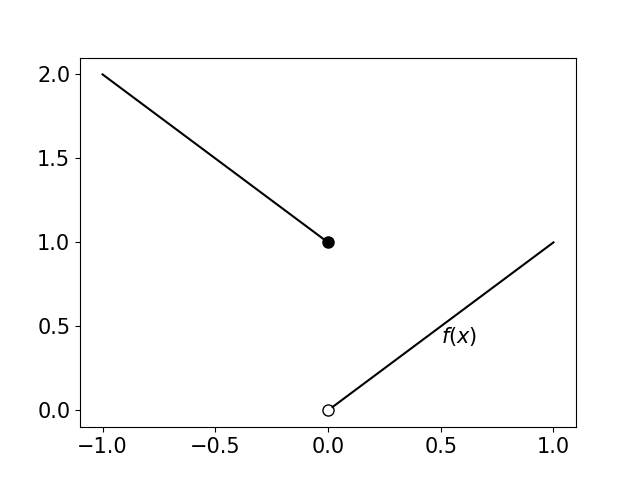
\includegraphics[width=0.4\textwidth]{figures/discontinuous_function.png}};
        \node at (7,0) {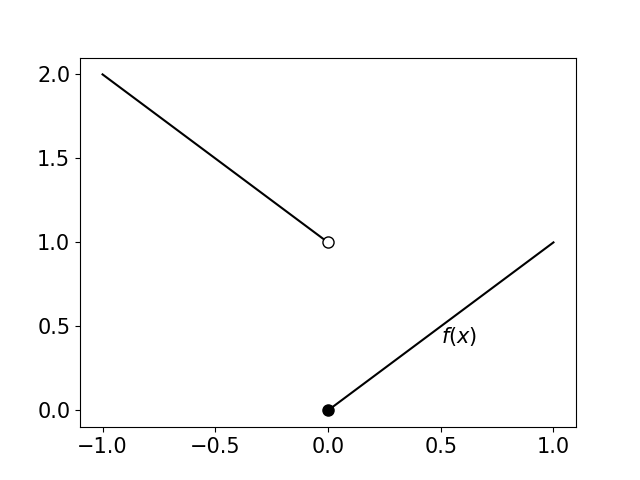
\includegraphics[width=0.4\textwidth]{figures/lsc_function.png}};
        \node at (0,-3) {No minimum attained};
        \node at (7,-3) {Minimum attained};
    \end{tikzpicture}
    \caption{Lack of lower-semicontinuity may lead to infima not being attained!}
    \label{prelim:fig:lsc}
\end{figure}

\begin{defn}[Coercive]
    We call $f:V\rightarrow \R$ coercive if 
    \begin{equation}
        \lim_{\|x\|\rightarrow\infty} f(x) = \infty.
    \end{equation}
\end{defn}


\begin{theorem}\label{preliminaries:thm:direct_method}
    Let $f:V\rightarrow (-\infty,\infty]$ be proper, coercive, and lsc and $V$ be finite-dimensional\footnote{This is not necessary but assumed to avoid more complicated arguments.}. Then $f$ admits a minimium on $V$.
\end{theorem}
\begin{proof}
    The proof follows the so-called \emph{direct method}.
    \paragraph{Step 1: Take a minimizing sequence}
    Let $(x_n)_n$ be a minimizing sequence\footnote{As an exercise: Why does such a sequence always exist?}, that is, 
    \begin{equation}
        \lim_n f(x_n) = \inf_{x\in V} f(x).
    \end{equation}
    \paragraph{Step 2: Bounedness of the sequence}
    Since $f$ is coercive, the minimizing sequence must be bounded. Indeed, assume the contrary. Then we can find a subsequence $(x_{n(k)})_k$ such that $\|x_{n(k)}\|\rightarrow\infty$. By coercivity, this implies
    \begin{equation}
        f(x_{n(k)})\rightarrow\infty
    \end{equation}
    which is a contradiction to
    \begin{equation}
        f(x_{n(k)})\rightarrow \inf f<\infty.
    \end{equation}
    \paragraph{Step 3: Apply a copmpactness argument to extract a convergent subsequence}
    From \cref{thm:bolzano} we know that every bounded sequence in a finite dimensional vector space admits a convergent subsequence. Thus, we can take such a subsequence $(x_{n(k)})_k$ with limit $\lim_kx_{n(k)}=\hat x$.
    \paragraph{Step 4: Conclude using lsc}
    By lsc of $f$ we obtain
    \begin{equation}
        f(\hat x) \leq \liminf_{k\rightarrow \infty}x_{n(k)} = \lim_n f(x_n) = \inf_x f(x) \leq f(\hat{x}).
    \end{equation}
\end{proof}